% Options for packages loaded elsewhere
\PassOptionsToPackage{unicode}{hyperref}
\PassOptionsToPackage{hyphens}{url}
\PassOptionsToPackage{dvipsnames,svgnames,x11names}{xcolor}
%
\documentclass[
  11pt,
  a4paper,
]{article}
\usepackage{amsmath,amssymb}
\usepackage{setspace}
\usepackage{iftex}
\ifPDFTeX
  \usepackage[T1]{fontenc}
  \usepackage[utf8]{inputenc}
  \usepackage{textcomp} % provide euro and other symbols
\else % if luatex or xetex
  \usepackage{unicode-math} % this also loads fontspec
  \defaultfontfeatures{Scale=MatchLowercase}
  \defaultfontfeatures[\rmfamily]{Ligatures=TeX,Scale=1}
\fi
\usepackage[]{mathpazo}
\ifPDFTeX\else
  % xetex/luatex font selection
\fi
% Use upquote if available, for straight quotes in verbatim environments
\IfFileExists{upquote.sty}{\usepackage{upquote}}{}
\IfFileExists{microtype.sty}{% use microtype if available
  \usepackage[]{microtype}
  \UseMicrotypeSet[protrusion]{basicmath} % disable protrusion for tt fonts
}{}
\makeatletter
\@ifundefined{KOMAClassName}{% if non-KOMA class
  \IfFileExists{parskip.sty}{%
    \usepackage{parskip}
  }{% else
    \setlength{\parindent}{0pt}
    \setlength{\parskip}{6pt plus 2pt minus 1pt}}
}{% if KOMA class
  \KOMAoptions{parskip=half}}
\makeatother
\usepackage{xcolor}
\usepackage[margin=1in]{geometry}
\usepackage{longtable,booktabs,array}
\usepackage{calc} % for calculating minipage widths
% Correct order of tables after \paragraph or \subparagraph
\usepackage{etoolbox}
\makeatletter
\patchcmd\longtable{\par}{\if@noskipsec\mbox{}\fi\par}{}{}
\makeatother
% Allow footnotes in longtable head/foot
\IfFileExists{footnotehyper.sty}{\usepackage{footnotehyper}}{\usepackage{footnote}}
\makesavenoteenv{longtable}
\usepackage{graphicx}
\makeatletter
\newsavebox\pandoc@box
\newcommand*\pandocbounded[1]{% scales image to fit in text height/width
  \sbox\pandoc@box{#1}%
  \Gscale@div\@tempa{\textheight}{\dimexpr\ht\pandoc@box+\dp\pandoc@box\relax}%
  \Gscale@div\@tempb{\linewidth}{\wd\pandoc@box}%
  \ifdim\@tempb\p@<\@tempa\p@\let\@tempa\@tempb\fi% select the smaller of both
  \ifdim\@tempa\p@<\p@\scalebox{\@tempa}{\usebox\pandoc@box}%
  \else\usebox{\pandoc@box}%
  \fi%
}
% Set default figure placement to htbp
\def\fps@figure{htbp}
\makeatother
\setlength{\emergencystretch}{3em} % prevent overfull lines
\providecommand{\tightlist}{%
  \setlength{\itemsep}{0pt}\setlength{\parskip}{0pt}}
\setcounter{secnumdepth}{-\maxdimen} % remove section numbering
\pagestyle{plain}
% definitions for citeproc citations
\NewDocumentCommand\citeproctext{}{}
\NewDocumentCommand\citeproc{mm}{%
  \begingroup\def\citeproctext{#2}\cite{#1}\endgroup}
\makeatletter
 % allow citations to break across lines
 \let\@cite@ofmt\@firstofone
 % avoid brackets around text for \cite:
 \def\@biblabel#1{}
 \def\@cite#1#2{{#1\if@tempswa , #2\fi}}
\makeatother
\newlength{\cslhangindent}
\setlength{\cslhangindent}{1.5em}
\newlength{\csllabelwidth}
\setlength{\csllabelwidth}{3em}
\newenvironment{CSLReferences}[2] % #1 hanging-indent, #2 entry-spacing
 {\begin{list}{}{%
  \setlength{\itemindent}{0pt}
  \setlength{\leftmargin}{0pt}
  \setlength{\parsep}{0pt}
  % turn on hanging indent if param 1 is 1
  \ifodd #1
   \setlength{\leftmargin}{\cslhangindent}
   \setlength{\itemindent}{-1\cslhangindent}
  \fi
  % set entry spacing
  \setlength{\itemsep}{#2\baselineskip}}}
 {\end{list}}
\usepackage{calc}
\newcommand{\CSLBlock}[1]{\hfill\break\parbox[t]{\linewidth}{\strut\ignorespaces#1\strut}}
\newcommand{\CSLLeftMargin}[1]{\parbox[t]{\csllabelwidth}{\strut#1\strut}}
\newcommand{\CSLRightInline}[1]{\parbox[t]{\linewidth - \csllabelwidth}{\strut#1\strut}}
\newcommand{\CSLIndent}[1]{\hspace{\cslhangindent}#1}
\usepackage{lineno} % add 
\usepackage{amsmath} % add 
\linenumbers % turns line numbering on 

% Allowing for landscape pages
\usepackage{lscape}
\newcommand{\blandscape}{\begin{landscape}}
\newcommand{\elandscape}{\end{landscape}}

% Left justification of the text: see https://www.sharelatex.com/learn/Text_alignment
% \usepackage[document]{ragged2e} % already in the latex template
\newcommand{\bleft}{\begin{flushleft}}
\newcommand{\eleft}{\end{flushleft}}


% Add Supplementary Tables and Figures
% Code from https://stackoverflow.com/a/51337664
\newcommand{\beginsupplement}{
  \setcounter{table}{0}  
  \renewcommand{\thetable}{S\arabic{table}}
  \setcounter{figure}{0} 
  \renewcommand{\thefigure}{S\arabic{figure}}
}



\usepackage{bookmark}
\IfFileExists{xurl.sty}{\usepackage{xurl}}{} % add URL line breaks if available
\urlstyle{same}
\hypersetup{
  pdftitle={Covariates selection in capture-recapture models using the Lasso},
  pdfauthor={Olivier Gimenez1*; Ian Renner},
  colorlinks=true,
  linkcolor={RoyalBlue},
  filecolor={Maroon},
  citecolor={Blue},
  urlcolor={RoyalBlue},
  pdfcreator={LaTeX via pandoc}}

\title{Covariates selection in capture-recapture models using the Lasso}
\author{Olivier Gimenez\textsuperscript{1}* \and Ian Renner}
\date{2026-07-21}

\begin{document}
\maketitle

\setstretch{2}
\small

\textsuperscript{1} CEFE, Univ Montpellier, CNRS, EPHE, IRD, Montpellier, France

\texttt{*} Corresponding author: \href{mailto:olivier.gimenez@cefe.cnrs.fr}{\nolinkurl{olivier.gimenez@cefe.cnrs.fr}}

\normalsize

\vspace{1cm}
\hrule

Explaining temporal variation in survival is a central goal of capture--recapture (CR) studies, and the growing availability of environmental covariates -- e.g.~from remote sensing -- means analysts increasingly face many, often correlated, candidate covariates. Standard covariate-selection tools (AIC- or stepwise-based procedures, or their Bayesian counterparts such as DIC, SSVS or RJMCMC) become impractical or unstable as the number of candidates grows, since the number of candidate models increases combinatorially. We propose to use the Lasso, a penalized-likelihood approach that shrinks regression coefficients and sets unimportant ones exactly to zero, to perform automatic covariate selection in CR survival models. We implement an adaptive Lasso applied to the likelihood of Cormack-Jolly-Seber (CJS) models, with the regularization parameter selected by BIC along a grid of penalty values. A simulation study spanning a range of sample sizes, detection probabilities, effect sizes, numbers of covariates and correlation structures shows that the Lasso recovers the correct subset of covariates {[}PLACEHOLDER: summarise headline performance from \texttt{scenario\_grid\_summary.csv}{]}, performing comparably to AIC-based selection. We illustrate the approach with a 16-year CR dataset on white storks (\emph{Ciconia ciconia}) breeding in France, in which survival is modelled as a function of rainfall at 10 weather stations in the wintering grounds (Sahel, West Africa); the Lasso selects {[}PLACEHOLDER: N{]} station(s), consistent with an independent analysis based on a prior PCA reduction of the same rainfall covariates. Because it operates directly on the likelihood, the approach extends naturally to CR models with several linked parameter sets (survival, detection, transition), where combinatorial model selection is especially costly.

\vspace{3mm}
\hrule
\vspace{5mm}

\emph{Keywords}: capture--recapture; covariate selection; Lasso; penalized likelihood; survival analysis; regularization

\newpage

\section{Introduction}\label{introduction}

Explaining variation in demographic parameters such as survival is a central objective of statistical ecology. Capture--recapture (CR) methods are the standard tool for this task: individuals are captured, marked and (imperfectly) re-observed over time, and survival is estimated while explicitly accounting for detection probability (\citeproc{ref-Lebreton1992}{Lebreton et al. 1992}). To relate survival to environmental or individual covariates, CR modelling is typically framed as a form of (generalized) regression, in which the temporal or individual variation in survival is explained by one or several covariates on the logit scale.

This regression-like framing runs into a practical difficulty as soon as the number of candidate covariates grows -- a situation that has become the norm rather than the exception with the increasing availability of environmental data from remote sensing, climate reanalysis products and biologging (e.g.~GPS). Analysts are then confronted with many, often correlated, candidate covariates, and typically do not know a priori which of them belong in the model. Including all of them inflates the number of parameters to estimate, which degrades precision and predictive performance; strong correlation among covariates further destabilizes numerical estimation {[}PLACEHOLDER: cite illustrative example / figure of correlated covariates, cf.~talk slide D2{]}.

Several strategies exist to select covariates in CR models. Analysts commonly reduce the covariate set a priori based on ecological reasoning and collinearity diagnostics, then compare a set of candidate models using information criteria such as AIC, or a stepwise procedure {[}PLACEHOLDER: refs{]}. Bayesian alternatives include DIC, stochastic search variable selection (SSVS) or reversible-jump MCMC (RJMCMC) {[}PLACEHOLDER: refs{]}. All of these approaches, however, require fitting and comparing a number of candidate models that grows combinatorially with the number of covariates (\(2^K\) models for \(K\) covariates), which quickly becomes impractical -- our case study below involves 10 candidate covariates, i.e.~1024 possible models for a single parameter, and this number multiplies further in CR models with several linked parameter sets (survival, detection, transition).

Here we explore an alternative route: instead of comparing discrete candidate models, we cast covariate selection as a continuous shrinkage problem. Penalized-likelihood methods add a penalty on the magnitude of regression coefficients to the likelihood being maximized; the Lasso {[}Least Absolute Shrinkage and Selection Operator{]} uses an \(L_1\) penalty that has the property of setting some coefficient estimates exactly to zero, thereby performing covariate selection and shrinkage simultaneously, within a single model fit along a grid of penalty values. Penalized-likelihood approaches related to the Lasso have already been used in ecology, in particular for occupancy models and for species distribution models combining multiple data sources, but -- to our knowledge -- not yet for covariate selection in CR survival models, which is the gap we address here.

In this paper, we adapt the (adaptive) Lasso to the likelihood of Cormack--Jolly--Seber (CJS) CR models to perform automatic selection of covariates on survival. We describe the method (Section \ref{methods}), evaluate its performance through a simulation study spanning a range of sample sizes, detection probabilities, numbers of covariates and correlation structures (Section \ref{simulations}), and illustrate it with a case study on the effect of Sahelian rainfall on the survival of white storks (\emph{Ciconia ciconia}) breeding in France (Section \ref{case-study}). We conclude with current limitations and extensions, including to CR models with multiple linked parameter sets and to occupancy models (Section \ref{discussion}).

\section{Methods}\label{methods}

\subsection{Capture--recapture likelihood}\label{capturerecapture-likelihood}

Consider a CJS model for \(n\) individually marked animals monitored over \(T\) capture occasions. Let \(\phi_t\) denote the probability that an individual alive just after occasion \(t\) survives to occasion \(t+1\), and \(p_t\) the probability that an individual alive at occasion \(t\) is detected. Survival is related to a set of \(K\) covariates through a logit link,
\[
\text{logit}(\phi_t) = \mathbf{x}_t^\top \boldsymbol{\beta},
\]
where \(\mathbf{x}_t\) is the covariate vector (including an intercept) associated with interval \(t\) and \(\boldsymbol{\beta} = (\beta_0, \beta_1, \ldots, \beta_K)^\top\) the corresponding regression coefficients; detection is modelled separately (e.g.~constant, or with its own covariates). The CJS likelihood \(L(\boldsymbol{\beta}, \boldsymbol{p} \mid \text{data})\) is the standard product-multinomial likelihood over the observed encounter histories {[}PLACEHOLDER: full expression / reference{]}.

\subsection{Ridge regression and the Lasso}\label{ridge-regression-and-the-lasso}

Penalized-likelihood estimation replaces maximization of the log-likelihood \(\ell(\boldsymbol{\beta})\) by maximization of \(\ell(\boldsymbol{\beta})\) subject to a constraint on the magnitude of \(\boldsymbol{\beta}\). Ridge regression constrains the \(L_2\) norm of the coefficients, \(\sum_{j=1}^K \beta_j^2 \le c\), which shrinks coefficients towards zero but essentially never sets them exactly to zero. The Lasso instead constrains the \(L_1\) norm, \(\sum_{j=1}^K |\beta_j| \le c\); geometrically, the \(L_1\) constraint region is a polytope with corners and flat faces, so that the point where the likelihood contours first touch the constraint region often falls exactly on a corner or edge, setting the corresponding coefficient(s) to zero. This is what makes the Lasso a covariate-selection device rather than a pure shrinkage device (unpenalized intercepts are excluded from the constraint, following standard practice and consistent with \texttt{unpenalised\_parameters} in \texttt{run\_casestudy.R}).

It is convenient to rewrite the constrained problem in Lagrangian form: for a penalty parameter \(\lambda \ge 0\), the Lasso estimate maximizes
\[
\ell(\boldsymbol{\beta}) - \lambda \sum_{j=1}^K w_j |\beta_j|,
\]
where we use an \emph{adaptive} Lasso with weights \(w_j = 1/|\hat\beta_j^{\text{MLE}}|^{\gamma}\) derived from the unpenalized (full) model fit, so that covariates with a larger unpenalized effect are penalized less. This construction gives the adaptive Lasso oracle properties: asymptotically, it recovers the correct subset of nonzero covariates with an optimal estimation rate.

\subsection{Choice of the regularization parameter}\label{choice-of-the-regularization-parameter}

The amount of shrinkage is governed by \(\lambda\). We adopt a grid-search (brute-force) strategy: the penalized likelihood is maximized over a grid of \(\lambda\) values {[}PLACEHOLDER: state grid range/spacing used, cf.~\texttt{lambda\_grid} in the scripts, e.g.~from \(10^{-3}\) to 100 on a log scale, 150 values{]}, and the retained model is the one minimizing the Bayesian Information Criterion,
\[
\text{BIC}(\lambda) = -2\,\ell(\hat{\boldsymbol{\beta}}_\lambda) + df_\lambda \log(n),
\]
where \(df_\lambda\) is the number of nonzero estimated coefficients (penalized and unpenalized) at \(\lambda\). We favour this grid/BIC approach over \(k\)-fold cross-validation because the latter requires refitting the whole path \(k\) times and, more importantly, because the value of \(\lambda\) needed to shrink all covariates to zero (\(\lambda_{\max}\)) can differ across folds, making the choice of a common \(\lambda\) grid across folds delicate.

\subsection{Implementation}\label{implementation}

The CJS likelihood, the adaptive-Lasso path and the BIC-based selection are implemented in R {[}PLACEHOLDER: package/functions -- \texttt{R/cjs\_likelihood.R}, \texttt{R/fit\_adaptive\_lasso.R}; optimization via \texttt{optim()}{]}. Coefficients are considered zero below a small numerical tolerance (\texttt{zero\_tolerance}) rather than exactly zero, as is typical of penalized likelihoods maximized with general-purpose optimizers rather than coordinate-descent algorithms {[}PLACEHOLDER: acknowledge/discuss discrepancy with true coordinate-descent Lasso solutions, cf.~talk comment on \texttt{optim} vs descent algorithms{]}.

\section{Simulation study}\label{simulations}

To evaluate the ability of the adaptive Lasso to recover the correct covariates and to compare its performance with AIC-based selection, we conducted a factorial simulation study {[}PLACEHOLDER: matches \texttt{run\_scenario\_grid.R}{]}.

\subsection{Design}\label{design}

We simulated CJS data under a full factorial design crossing:

\begin{itemize}
\tightlist
\item
  number of capture occasions: \(T \in \{10, 15, 20\}\),
\item
  number of newly marked individuals per occasion: \(\{10, 20\}\),
\item
  mean survival: \(\bar\phi = 0.8\),
\item
  detection probability: \(p \in \{0.5, 0.9\}\),
\item
  effect size of the informative covariates (on the logit scale): \(\{-0.3, -0.6\}\),
\item
  number of candidate covariates: \(\{5, 10, 20\}\), of which \(2\) are truly informative (\texttt{n\_active\ =\ 2}) and the remainder are noise covariates,
\item
  pairwise correlation among covariates: \(\{0, 0.5, 0.8\}\).
\end{itemize}

Each of the resulting scenarios was replicated 100 times {[}PLACEHOLDER: total number of scenarios \(\times\) replicates; seed = 20260720 for reproducibility{]}. For each simulated dataset we (i) fitted the adaptive-Lasso path over a grid of \(\lambda \in [10^{-3}, 100]\) (150 values) and selected \(\lambda\) by BIC, and (ii) where feasible, fitted all \(2^K\) candidate models and selected the best one by AIC, for comparison.

\subsection{Performance metrics}\label{performance-metrics}

We assessed performance in terms of: (i) the proportion of replicates in which the Lasso selected exactly the correct subset of covariates (true positives only), (ii) sensitivity (proportion of truly informative covariates retained) and specificity (proportion of noise covariates correctly excluded), and (iii) how these metrics varied with sample size, detection probability, effect size, number of candidate covariates and correlation strength; AIC-based selection was used as a benchmark where computationally tractable (i.e.~for the smaller covariate sets).

\subsection{Results}\label{results}

{[}PLACEHOLDER: to be filled from \texttt{scenario\_grid\_summary.csv} / \texttt{simulation\_covariate\_selection.csv}. As reported in the preliminary talk on a simpler 2-covariate design, the Lasso recovered the correct model in about 80\% of replicates, comparable to AIC; the fuller factorial design here should let us describe how this performance changes with the number of covariates, correlation, detection probability and effect size -- e.g.~a figure with selection performance on the y-axis against number of covariates, faceted by correlation and detection probability, analogous to \texttt{plot\_selection\_performance()}.{]}

\section{Case study: white stork survival and Sahelian rainfall}\label{case-study}

\subsection{Data}\label{data}

We illustrate the approach with a long-term CR dataset on white storks breeding in France {[}PLACEHOLDER: precise site/region, ref to original data source/publication{]}. The dataset spans 16 years and includes more than 200 individually marked birds. White storks breeding in France winter in the Sahel region of West Africa, where rainfall is thought to affect survival through its influence on food availability. We considered rainfall measured at 10 weather stations across the Sahel as candidate covariates on adult survival, together with a survival intercept and a (constant, or PLACEHOLDER) detection model.

\subsection{Motivation for the Lasso}\label{motivation-for-the-lasso}

With 10 candidate rainfall covariates, an AIC-based model-selection approach on survival alone would require comparing \(2^{10} = 1024\) candidate models. We instead fitted the full model (intercept plus all 10 station covariates) and applied the adaptive-Lasso path described above.

\subsection{Results}\label{results-1}

{[}PLACEHOLDER: populate with actual output of \texttt{run\_casestudy.R} -- \texttt{whitestork\_lasso\_coefficients.csv} / \texttt{whitestork\_lasso\_results.rds}.{]} The BIC criterion, computed along the \(\lambda\) grid, was minimized around \(\lambda \approx 0.05\) (Fig. \ref{fig:bic-path}; cf.~\texttt{plot\_lasso\_criterion()}). Tracking individual coefficient paths as \(\lambda\) increases (Fig. \ref{fig:coef-path}; cf.~\texttt{plot\_lasso\_path()}) shows that all but one coefficient are shrunk to zero before reaching the selected \(\lambda\). At the selected \(\lambda\), only the covariate for the {[}PLACEHOLDER: station name, e.g.~Kita{]} station retains a nonzero, {[}PLACEHOLDER: sign{]} estimate (Table \ref{tab:coef-table}; cf.~\texttt{coefficient\_table} / \texttt{selected\_covariates}). This is consistent with an earlier analysis of overlapping rainfall data that first reduced the 10 stations to a single axis by PCA before fitting the CR model {[}PLACEHOLDER: cite that earlier study{]}.

\begin{figure}

{\centering 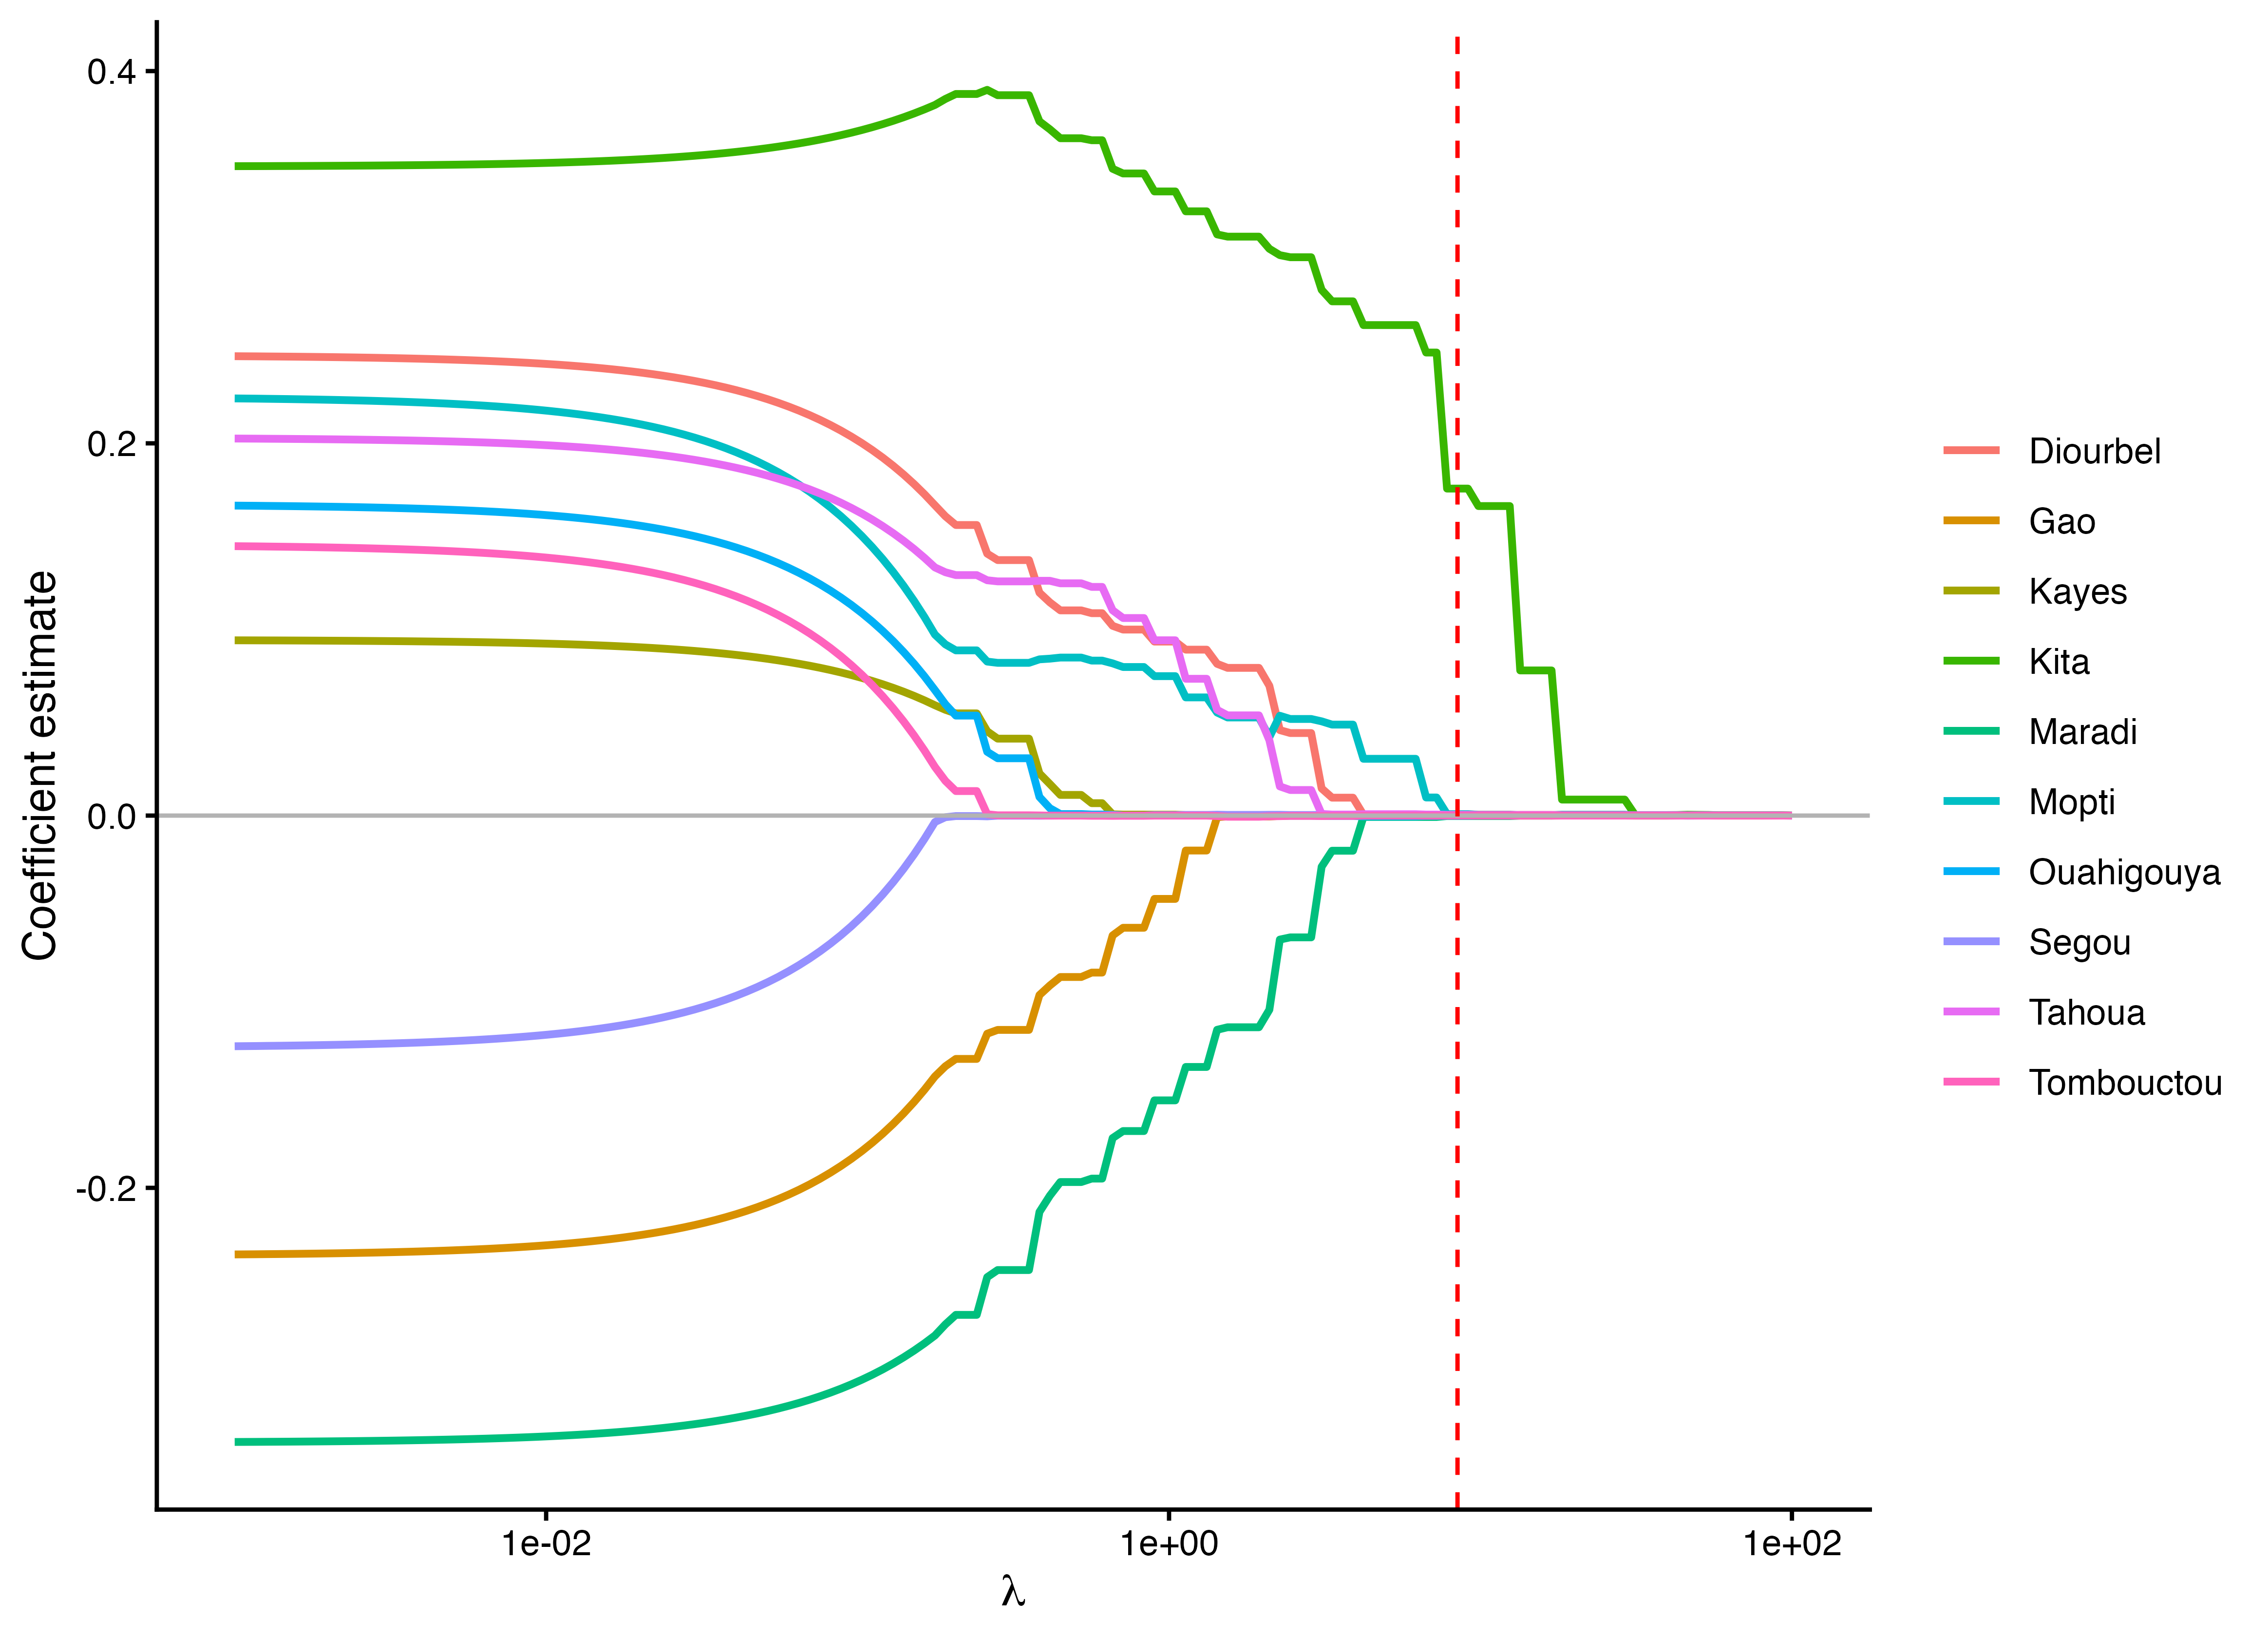
\includegraphics[width=1\linewidth]{path_stork} 

}

\caption{Regularization paths for the 10 rainfall-station coefficients; vertical line: BIC-selected lambda.}\label{fig:coef-path}
\end{figure}

\section{Discussion}\label{discussion}

We have shown that the (adaptive) Lasso, applied directly to the CJS likelihood, provides an effective alternative to information-criterion-based or Bayesian variable-selection procedures for covariate selection in CR survival models, at a fraction of the computational cost, since it avoids fitting and comparing a combinatorially large set of candidate models.

A key advantage of working directly at the likelihood level is that the approach generalizes readily to CR models with several linked sets of parameters -- for instance multistate models (survival, detection, transition probabilities) or multievent models with additional latent-state parameters -- where combinatorial model selection across parameter sets is particularly cumbersome (which set of covariates to test first, and in which order?). The Lasso sidesteps this question entirely by penalizing all parameter sets jointly within a single model fit. Modifying existing CR software to implement a penalized likelihood is comparatively straightforward, which suggests the approach could in time be incorporated into standard CR platforms (e.g.~MARK, \texttt{unmarked}, E-SURGE) {[}PLACEHOLDER: confirm claim/tone{]}.

Several limitations remain. First, our current implementation does not provide confidence intervals or significance tests for the selected coefficients; the bootstrap is a natural solution but increases computation time substantially, and its performance under adaptive-Lasso shrinkage remains to be characterized. Second, we focused on continuous, purely temporal covariates; when covariates are categorical (e.g.~age class or discrete time effects), one is often not interested in the effect of a single level but in the effect of the \emph{factor as a whole}, which the plain Lasso does not handle naturally -- the group Lasso, which penalizes and selects groups of coefficients jointly, is a natural extension we are currently exploring. Third, our optimizer (\texttt{optim()}) yields coefficients that are shrunk close to, but not always exactly at, zero, unlike coordinate-descent algorithms designed specifically for the Lasso; a numerical zero-tolerance threshold is used here as a practical workaround, but implementing a dedicated descent algorithm (requiring the CJS score equations) would be a cleaner long-term solution {[}PLACEHOLDER: decide whether to keep this as a stated limitation or to actually implement it before submission{]}.

Finally, penalized-likelihood approaches related to the Lasso already exist for occupancy models, and we see an opportunity to connect that literature with the CR setting explored here, including a Bayesian formulation of the shrinkage prior underlying the Lasso {[}PLACEHOLDER: cf.~talk perspective ``give a Bayesian flavour to the whole thing''{]}.

\section{Acknowledgments}\label{acknowledgments}

{[}PLACEHOLDER: acknowledgments specific to this project -- the current text mentions collaborators from an unrelated otter/spatial-stream-network project and should not be reused here.{]}

\subsection{Data availability statement}\label{data-availability-statement}

{[}PLACEHOLDER: per JSE guidelines, code and data (or a fully reproducible simulated look-alike dataset, if the white stork data cannot be shared openly) must be archived, e.g.~on GitHub/Zenodo, with an anonymized link at submission for double-blind review -- see \url{https://anonymous.4open.science/}.{]}

\subsection{Funding statement}\label{funding-statement}

{[}PLACEHOLDER{]}

\section{References}\label{references}

\phantomsection\label{refs}
\begin{CSLReferences}{1}{0}
\bibitem[\citeproctext]{ref-Lebreton1992}
Lebreton, J.-D., K. P. Burnham, J. Clobert, and D. R. Anderson. 1992. \href{https://doi.org/10.2307/2937171}{Modeling survival and testing biological hypotheses using marked animals: A unified approach with case studies}. Ecological Monographs 62:67--118.

\end{CSLReferences}

\clearpage

\newpage

\end{document}
